\documentclass{beamer}
\usetheme[sectionpage=none]{metropolis}

\usepackage{tikz}
\usepackage{tkz-graph}
\usetikzlibrary{calc,shapes.multipart,chains,arrows,backgrounds}

\usepackage{minted}
\setminted[haskell]{escapeinside=@@}
\newcommand{\hs}{\mintinline{haskell}}

\usepackage{mathtools}

\renewcommand{\epsilon}{\varepsilon}
\newcommand{\eps}{\epsilon}
\newcommand{\connect}{\rightarrow}


\title{Algebraic Graphs with Class}
\author{Christoph Madlener}
\date{01.06.2021}

\begin{document}
\begin{frame}[plain]
  \titlepage
\end{frame}

\section{Introduction}
\begin{frame}[fragile]
  \frametitle{Introduction}

  \begin{columns}
    \begin{column}{.6\linewidth}
      \onslide<1->
      \centering
      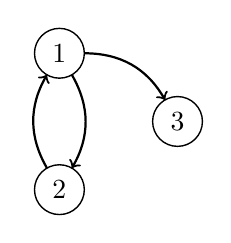
\begin{tikzpicture}
        \tikzset{EdgeStyle/.style = {->, bend left}}
        \Vertices{circle}{3,1,2}
        \Edge(1)(2)
        \Edge(2)(1)
        \Edge(1)(3)
      \end{tikzpicture}
      $G_1$\onslide<3->${} = \Big(\big\{1,2,3\big\}, \big\{(1,2), (1,3), (2,1)\big\}\Big)$
    \end{column}
    \begin{column}{.35\linewidth}
      \onslide<2->
      \[
        G = (V,E) \text{ s.t. } \alert{E \subseteq V \times V}
      \]
    \end{column}
  \end{columns}

  \onslide<4->
  \begin{alertblock}{In Haskell?}
    \begin{minted}{haskell}
    data G a = G { vs :: Set a, es :: Set (a,a) }
    \end{minted}
    \onslide<5->
    \hs{g1 = G [1,2,3] [(1,2), (1,3), (2,1)]} 
    \onslide<6->
    \hs{g2 = G [1,2] [(1,3)]} \hspace{15mm}{\color{red} $E \nsubseteq V \times V$}
  \end{alertblock}
\end{frame}


\begin{frame}
  \frametitle{\texttt{containers} \& \texttt{fgl}}
  \begin{columns}[t]
    \begin{column}{.35\textwidth}
      \onslide<+->
      \begin{exampleblock}{\texttt{containers}}
        adjacency lists
        
        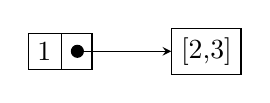
\begin{tikzpicture}[vertex/.style={rectangle split, rectangle split parts=2,
            draw, rectangle split horizontal}, >=stealth, start chain,
          list/.style={rectangle,draw}]

          \node[vertex,on chain] (1) {1};
          \node[list,on chain] (2) {[2,3]};
          \draw[*->] let \p1 = (1.two), \p2 = (1.center) in (\x1,\y2) -- (2);
        \end{tikzpicture}
        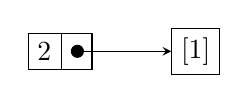
\begin{tikzpicture}[vertex/.style={rectangle split, rectangle split parts=2,
            draw, rectangle split horizontal}, >=stealth, start chain,
          list/.style={rectangle,draw}]

          \node[vertex,on chain] (1) {2};
          \node[list,on chain] (2) {[1]};
          \draw[*->] let \p1 = (1.two), \p2 = (1.center) in (\x1,\y2) -- (2);
        \end{tikzpicture}
        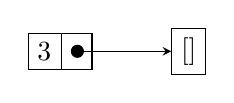
\begin{tikzpicture}[vertex/.style={rectangle split, rectangle split parts=2,
            draw, rectangle split horizontal}, >=stealth, start chain,
          list/.style={rectangle,draw}]

          \node[vertex,on chain] (1) {3};
          \node[list,on chain] (2) {[]};
          \draw[*->] let \p1 = (1.two), \p2 = (1.center) in (\x1,\y2) -- (2);
        \end{tikzpicture}
      \end{exampleblock}
    \end{column}
    \begin{column}{.55\textwidth}
      \onslide<+->
      \begin{exampleblock}{\texttt{fgl}}
        \textit{inductive graphs}
        \begin{itemize}
        \item inductive datatype: Context of a vertex + Graph
        \end{itemize}
      \end{exampleblock}
    \end{column}
  \end{columns}
  \onslide<+->
  
  \begin{alertblock}{$E \subseteq V \times V$ ?}
    \onslide<+->
    \begin{itemize}
    \item partial functions \textrightarrow runtime errors
    \end{itemize}
  \end{alertblock}
\end{frame}

\begin{frame}[fragile]
  \frametitle{Algebraic Graphs}
  \onslide<+->
  \begin{itemize}
  \item complete and \alert{consistent} graph representation
  \item simple construction primitives (\emph{``the core''})
  \end{itemize}
  \onslide<+->
  \begin{alertblock}{Achieved by the datatype}
    \begin{minted}{haskell}
    data Graph a = Empty
                 | Vertex a
                 | Overlay (Graph a) (Graph a)
                 | Connect (Graph a) (Graph a)
    \end{minted}
  \end{alertblock}
\end{frame}

\begin{frame}
  \frametitle{Empty ($\eps$) \& Vertex}
  \begin{columns}[t]
    \onslide<+->
    \begin{column}{.45\textwidth}
      \begin{exampleblock}{Empty - $\eps$}
        \vspace{5pt}
        \centering 
        \begin{tikzpicture}
          \draw[draw=black,fill=mDarkTeal!30] (0,0) rectangle ++ (3,3);
        \end{tikzpicture}
        
        \hs{Empty} ${} = \eps = (\emptyset, \emptyset)$
      \end{exampleblock}
    \end{column}
    \onslide<+->
    \begin{column}{.45\textwidth}
      \begin{exampleblock}{Vertex}
        \vspace{5pt}
        \centering
        \begin{tikzpicture}
          \draw[draw=black,fill=mDarkTeal!30] (0,0) rectangle ++ (3,3);
          \Vertex[x=1.5,y=1.5]{1};
        \end{tikzpicture}

        \hs{Vertex 1} ${} = (\{1\}, \emptyset)$
      \end{exampleblock}
    \end{column}
  \end{columns}
\end{frame}

\begin{frame}
  \frametitle{Overlay ($+$)}
  \begin{columns}[b]
    \begin{column}{.25\textwidth}
      \centering
      \begin{tikzpicture}[background rectangle/.style={fill=mDarkTeal!30,draw=black},
        show background rectangle]
        \Vertices{tr4}{3,2,1};
        \Edge[style={bend right,->}](1)(2);
        \Loop[dir=SOEA, dist=0.8cm](3);
      \end{tikzpicture}
    \end{column}
    \begin{column}{.1\textwidth}
      \centering
      {\LARGE $+$}
      \vspace{13mm}
    \end{column}
    \begin{column}{.25\textwidth}
      \centering
      \begin{tikzpicture}[background rectangle/.style={fill=mDarkTeal!30,draw=black},
        show background rectangle]
        \Vertices{line}{2,3};
        \Edge[style={bend right,->}](2)(3);
        \Loop[dir=SOEA, dist=0.8cm](3);
      \end{tikzpicture}
    \end{column}
    \begin{column}{.1\textwidth}
      \centering
      {\LARGE $=$}
      \vspace{13mm}
    \end{column}
    \begin{column}{.25\textwidth}
      \centering
      \begin{tikzpicture}[background rectangle/.style={fill=mDarkTeal!30,draw=black},
        show background rectangle]
        \Vertices{tr4}{3,2,1};
        \Edge[style={bend right,->}](1)(2);
        \Edge[style={bend right,->}](2)(3);
        \Loop[dir=SOEA, dist=0.8cm](3);
      \end{tikzpicture}
    \end{column}
  \end{columns}
  \[
    (V_1, E_1) + (V_2, E_2) \coloneqq (V_1 \cup V_2, E_1 \cup E_2)
  \]
\end{frame}

\begin{frame}
  \frametitle{Connect ($\connect$ / $*$)}
  \begin{columns}[b]
    \begin{column}{.25\textwidth}
      \centering
      \begin{tikzpicture}[background rectangle/.style={fill=mDarkTeal!30,draw=black},
        show background rectangle]
        \Vertex[x=0,y=1]{1};
        \Vertex[x=0,y=0]{2};
        \Edge[style={bend right,->}](1)(2);
      \end{tikzpicture}
    \end{column}
    \begin{column}{.1\textwidth}
      \centering
      {\LARGE $\connect$}
      \vspace{7mm}
    \end{column}
    \begin{column}{.25\textwidth}
      \centering
      \begin{tikzpicture}[background rectangle/.style={fill=mDarkTeal!30,draw=black},
        show background rectangle]
        \Vertex[x=0,y=1]{1};
        \Vertex[x=1,y=0]{3};
        \Edge[style={bend left,->}](1)(3);
      \end{tikzpicture}
    \end{column}
    \begin{column}{.1\textwidth}
      \centering
      {\LARGE $=$}
      \vspace{7mm}
    \end{column}
    \begin{column}{.25\textwidth}
      \centering
      \begin{tikzpicture}[background rectangle/.style={fill=mDarkTeal!30,draw=black},
        show background rectangle]
        \Vertex[x=0,y=1]{1};
        \Vertex[x=0,y=0]{2};
        \Vertex[x=1,y=0]{3};
        \Loop[dist=0.8cm](1)
        \Edge[style={bend left,->}](1)(3);
        \tikzset{EdgeStyle/.style={bend right,->}}
        \Edge(1)(2);
        \Edge(2)(1);
        \Edge(2)(3);
      \end{tikzpicture}
    \end{column}
  \end{columns}
  \[
    (V_1, E_1) \connect (V_2, E_2) \coloneqq (V_1 \cup V_2, E_1 \cup E_2 \cup
    V_1 \times V_2)
  \] 
\end{frame}

\section{Graph Construction \& Transformation}
\begin{frame}
  \frametitle{Graph Construction}
  
\end{frame}

\begin{frame}
  \frametitle{Graph Transformation}
  
\end{frame}

\section{Algebra}
\begin{frame}
  \frametitle{\textsc{Algebraic} Graphs with \textsc{Class}}
\end{frame}

\begin{frame}
  \frametitle{Undirected Graphs \& more}
  
\end{frame}

\begin{frame}
  \frametitle{Formal Verification}
  
\end{frame}

\section{Deep Embedding}
\begin{frame}
  \frametitle{Deep Embedding}
  
\end{frame}

\begin{frame}
  \frametitle{Formal Verification}
  
\end{frame}

\section{Conclusion}
\begin{frame}
  \frametitle{Conclusion}
  
\end{frame}
\end{document}